\documentclass[12pt,a4paper]{article}

% Packages
\usepackage[utf8]{inputenc}
\usepackage[T1]{fontenc}
\usepackage{amsmath,amssymb,amsthm}
\usepackage{graphicx}
\usepackage{booktabs}
\usepackage{hyperref}
\usepackage[margin=2.5cm]{geometry}
\usepackage{setspace}
\usepackage{natbib}
\usepackage{float}
\usepackage{caption}
\usepackage{subcaption}
\usepackage{tikz}
\usepackage{pgfplots}
\pgfplotsset{compat=1.18}
\usepackage{longtable}
\usepackage{pdflscape}
\usepackage{xcolor}
\usepackage{textcomp}
\usepackage{tgtermes}

% Custom colors
\definecolor{btcorange}{RGB}{247,147,26}
\definecolor{mstrblue}{RGB}{0,82,147}

% Line spacing
\onehalfspacing

% Hyperref setup
\hypersetup{
    colorlinks=true,
    linkcolor=mstrblue,
    citecolor=mstrblue,
    urlcolor=mstrblue
}

% Title
\title{%
    \textbf{Long Vol, Long BTC, Long Saylor} \\[0.5cm]
    \large Analyzing MicroStrategy's Reflexive Feedback Loop: \\
    Capital Structure, Convertible Arbitrage, and Bitcoin Acquisition Strategy
}

\author{%
    Dave Montali\footnote{dave.montali@hec.edu} \\
    Executive MSc in Finance \\
    HEC Paris \\[0.3cm]
    \small Supervisor: Co-Pierre Georg
}

\date{February 2026}

\begin{document}

\maketitle
\thispagestyle{empty}
\newpage

% Abstract
\begin{abstract}
\noindent
This thesis investigates the self-reinforcing feedback loop between Strategy's (MSTR) financing strategy and Bitcoin acquisitions. As of January 2026, Strategy holds 713,502 BTC financed through \$7.4 billion in convertible debt and \$8.5 billion in preferred shares. Using an event study around capital raises (August 2020 to January 2026), I document patterns consistent with reflexive capital formation: Strategy systematically raises capital during elevated premium windows. I analyze the capital structure through scenario analysis and examine how convertible arbitrageurs profit from the structure at the expense of retail equity holders.

\vspace{0.5cm}
\noindent\textbf{Keywords:} Strategy, MicroStrategy, Bitcoin, Convertible Bonds, Reflexivity, Capital Structure
\end{abstract}
\newpage

% Table of Contents
\tableofcontents
\newpage

% List of Figures and Tables
\listoffigures
\listoftables
\newpage

% Chapters
\section{Introduction}
\label{sec:introduction}

Strategy (formerly MicroStrategy, rebranded February 2025) announced its first Bitcoin purchase in August 2020: 21,454 BTC for roughly \$250 million. What began as an unconventional treasury allocation has since grown into the most aggressively leveraged cryptocurrency position ever assembled by a public company. By January 2026, Strategy held 713,502 Bitcoin with a cost basis of approximately \$54.3 billion, acquired through a financing strategy that would make most CFOs nervous and most academics skeptical.\footnote{All figures as of late January 2026 unless otherwise noted. The company trades under the ticker MSTR on NASDAQ. I use ``Strategy'' and ``MSTR'' interchangeably throughout.}

The conventional story treats MSTR as a simple Bitcoin proxy, a way for equity investors to gain exposure without holding the asset directly. This framing misses the more interesting dynamics at play. MSTR isn't just holding Bitcoin; it has engineered a capital structure designed to amplify returns in both directions while extracting value through financial engineering that rewards certain stakeholders at the expense of others.

I document conditional feedback dynamics consistent with what George Soros termed market reflexivity. The hypothesized loop works as follows: elevated stock prices enable cheap equity issuance; cheap equity funds Bitcoin purchases; Bitcoin purchases increase net asset value; higher NAV supports the stock price. The cycle persists as long as three conditions hold: access to capital markets, elevated implied volatility, and stable or rising Bitcoin prices. When any of these constants fails, the flywheel breaks. The empirical question is whether MSTR's behavior exhibits patterns consistent with this mechanism, and under what conditions the feedback operates.

This thesis examines four questions:

\begin{enumerate}
    \item How has MicroStrategy's financing strategy created a self-reinforcing feedback loop between its stock price, volatility, and Bitcoin accumulation?
    \item What is the quantitative relationship between MSTR's NAV premium and subsequent capital raising?
    \item How do convertible bond arbitrageurs amplify the reflexivity mechanism, and what does this mean for different investor classes?
    \item Under what conditions does the flywheel break, and who bears the losses when it does?
\end{enumerate}

\subsection{Hypotheses}

\textbf{H1:} MicroStrategy's NAV premium exhibits a statistically significant positive relationship with subsequent Bitcoin purchases, consistent with reflexive feedback.

\textbf{H2:} The self-reinforcing loop requires three conditions to persist: continuous capital raising capability, elevated implied volatility, and rising or stable Bitcoin prices.

\textbf{H3:} Retail equity investors face asymmetric downside risk compared to convertible arbitrageurs, who extract value through gamma scalping while maintaining hedged positions.

\subsection{Contribution}

The existing literature treats reflexivity as a qualitative concept, applies Merton models to traditional corporate assets, and examines convertible arbitrage in isolation. This thesis integrates all three frameworks to analyze a structure that didn't exist before 2020.

I contribute in three ways. First, I document patterns consistent with reflexive capital formation at the firm level using an event study around capital raises. While \citet{soros1987alchemy} offers theoretical insight without mathematical specification, I test whether MSTR's behavior exhibits observable patterns consistent with reflexive dynamics. The evidence shows that Strategy systematically raises capital during elevated premium windows, and that the premium exhibits extreme persistence rather than mean-reversion. Second, I frame MSTR equity as a call option on Bitcoin and analyze the capital structure through breakeven prices and asset/debt ratios rather than Merton model outputs that assume away Bitcoin's defining characteristics. Third, I describe how convertible arbitrageurs extract value from the structure through gamma scalping while retail equity holders bear leveraged directional risk.

The remainder of this section reviews the relevant literature. Subsequent sections cover capital structure analysis, methodology, results, discussion with comparative evidence from other Digital Asset Treasury Companies (DATCOs), and conclusion.

\section{Literature Review}
\label{sec:literature}

Three strands of academic work inform this analysis: market reflexivity, structural credit models, and convertible bond arbitrage. None adequately addresses the phenomenon MSTR represents, but together they provide the theoretical scaffolding for understanding what the company has built.

\subsection{Market Reflexivity}

George Soros introduced reflexivity in \textit{The Alchemy of Finance} \citep{soros1987alchemy}, arguing that market participants don't merely observe fundamentals but actively shape them. Prices reflect beliefs about value, and those beliefs influence the very fundamentals they purport to measure. Two functions operate simultaneously: a cognitive function where participants try to understand the world, and a participating function where their actions change it. When both functions interact, self-reinforcing cycles emerge that deviate from equilibrium predictions.

The standard critique of reflexivity is that it's unfalsifiable. If markets go up, reflexivity explains the feedback loop. If markets go down, reflexivity explains the reversal. Soros never provides a mathematical specification that would allow empirical testing. \citet{shiller2015irrational} documents feedback trading in equity markets and offers survey evidence of extrapolative expectations, but his work focuses on market-wide dynamics rather than firm-level mechanisms. \citet{brunnermeier2014macroeconomic} models amplification in credit markets through leverage constraints, showing how falling asset prices tighten funding conditions, which forces asset sales, which depresses prices further. Their framework is rigorous but operates at the macro level.

I contend that MSTR offers a unique laboratory for testing whether firm-level dynamics exhibit patterns consistent with reflexivity, where each link in the hypothesized chain is observable. The proposed mechanism operates through concrete channels: stock price determines equity issuance capacity; issuance capacity determines Bitcoin accumulation; Bitcoin holdings determine net asset value; NAV influences stock price. Each link can be measured:
\begin{enumerate}
    \item High stock price $\rightarrow$ cheap equity capital
    \item Cheap capital $\rightarrow$ more BTC purchases
    \item More BTC $\rightarrow$ higher NAV
    \item Higher NAV $\rightarrow$ higher stock price
\end{enumerate}

Rather than claim to prove reflexivity exists, I test whether observable patterns are consistent with reflexive dynamics. The contribution is methodological: providing a framework for measuring feedback loops in corporate finance contexts, with MSTR as the test case. Whether these patterns constitute ``reflexivity'' in Soros's philosophical sense is less important than whether they have predictive content for understanding MSTR's capital formation behavior.

\subsection{Merton Structural Credit Model}

\citet{merton1974pricing} transformed credit analysis by recognizing that equity is a call option on firm assets. Shareholders receive the residual after debt is paid: $\max(V_T - D, 0)$ at maturity, where $V_T$ is asset value and $D$ is debt face value. Debt holders receive $\min(V_T, D)$. This insight allows Black-Scholes-Merton pricing:
\begin{align}
    E &= V \cdot N(d_1) - D \cdot e^{-rT} \cdot N(d_2) \\
    d_1 &= \frac{\ln(V/D) + (r + \sigma^2/2)T}{\sigma\sqrt{T}} \\
    d_2 &= d_1 - \sigma\sqrt{T}
\end{align}

The distance to default measures how many standard deviations separate current asset value from the default threshold:
\begin{equation}
    DD = \frac{\ln(V/D) + (\mu - \sigma^2/2)T}{\sigma\sqrt{T}}
\end{equation}

Critics note that Merton models systematically underpredict credit spreads (the ``credit spread puzzle''), and that the lognormal assumption poorly captures fat-tailed asset distributions. \citet{leland1994corporate} extends the framework to incorporate optimal capital structure, and \citet{collin2001determinants} applies it to spread prediction with mixed success.

MSTR presents an unusually clean test case for the Merton framework, cleaner than most corporate applications. The asset (Bitcoin) has continuous market prices with no estimation required. Volatility can be calculated directly from BTC returns rather than backed out from equity prices. The debt structure is publicly documented. And equity trades continuously, allowing real-time model validation. The challenge is that Bitcoin's volatility exceeds anything Merton contemplated, raising questions about how the framework behaves at extreme parameter values.

\subsection{Convertible Bond Arbitrage}

Convertible bonds combine straight debt with an embedded equity call option. The classic arbitrage strategy, documented by \citet{agarwal2011convertible}, involves buying the convertible, shorting the underlying equity to hedge delta, and profiting from volatility through gamma scalping. As the stock moves, the delta of the embedded option changes, requiring hedge rebalancing. This rebalancing generates trading profits proportional to realized volatility.

The relevant Greeks for convertible arbitrage are delta (sensitivity to underlying price), gamma (rate of delta change, determining rebalancing frequency), vega (sensitivity to implied volatility), and theta (time decay). \citet{choi2009convertible} show that convertible arb funds are net providers of delta hedging flow, and their activity can amplify rather than dampen stock volatility. When gamma is large (at-the-money converts), even small price moves trigger significant hedging trades.

\citet{shleifer1997limits} complicate the arbitrage picture by demonstrating that capital constraints, agency problems, and noise trader risk prevent arbitrageurs from fully exploiting mispricings. Arbitrage isn't frictionless. Positions require capital and entail risks beyond the textbook spread. In the MSTR context, this suggests that even sophisticated arb funds face constraints that may allow the NAV premium to persist longer than pure efficiency would predict.

MSTR amplifies convertible arb dynamics because the notional outstanding is large relative to equity float, underlying Bitcoin volatility exceeds typical equity vol by a factor of two or three, and the zero-coupon structure maximizes the embedded option component. These characteristics suggest that convertible arbitrageurs are well-positioned to extract value from the structure regardless of Bitcoin's direction.

\subsection{Cryptocurrency Markets and Corporate Adoption}

The academic literature on crypto markets has grown rapidly since Bitcoin's inception. \citet{liu2022risks} establish that cryptocurrency returns are driven by factors distinct from traditional asset pricing models; network effects and momentum dominate. \citet{makarov2020trading} document substantial cross-exchange arbitrage opportunities, suggesting persistent inefficiencies. \citet{griffin2020bitcoin} raise concerns about price manipulation, though the extent remains debated.

Corporate Bitcoin adoption is a newer phenomenon with limited academic coverage. \citet{baker2022corporate} survey post-2020 treasury practices and find increased interest in digital assets as inflation hedges. \citet{yi2021bitcoin} examine announcement effects of corporate Bitcoin purchases on stock returns. But MicroStrategy sits outside the scope of this literature. Most corporate adopters allocated single-digit percentages of treasury to Bitcoin. MSTR made it the entire balance sheet. No framework exists for analyzing a company that has transformed itself from a software firm into a leveraged Bitcoin vehicle. Since 2024, a growing cohort of public companies have adopted variants of Strategy's model, collectively referred to as Digital Asset Treasury Companies (DATCOs). I examine these firms comparatively in Section~\ref{sec:datco_landscape}.

\subsection{Research Gap}

The literatures on reflexivity, credit modeling, and convertible arbitrage developed independently and address different phenomena. Soros wrote about macro markets, Merton about corporate debt, and the arb literature about hedge fund strategies. No prior work has tested for reflexive dynamics in a single-issuer cryptocurrency context, applied structural credit models to crypto-backed liabilities, or modeled how convertible arbitrage interacts with firm-level feedback loops.

This thesis addresses that gap by integrating the three frameworks. The MSTR structure offers what approaches a natural experiment: a publicly traded company whose capital structure makes the hypothesized feedback mechanism observable and, within the limits of non-experimental data, testable.


\section{Strategy's Capital Structure}
\label{sec:capital_structure}

Strategy has built something that resembles a synthetic collateralized debt obligation, except with a single underlying asset. Traditional CDOs derive whatever stability they have from pooling uncorrelated assets; MSTR offers only the appearance of diversification through seniority. Every tranche, from senior convertible debt to junior preferred shares to common equity, is backed by the same thing: Bitcoin. When BTC falls, everyone falls together. The seniority waterfall determines only the order in which different investors get wiped out, not whether they avoid exposure to the underlying risk.

Figure~\ref{fig:capital_structure} illustrates the hierarchy of claims as of January 2026.

\begin{figure}[H]
    \centering
    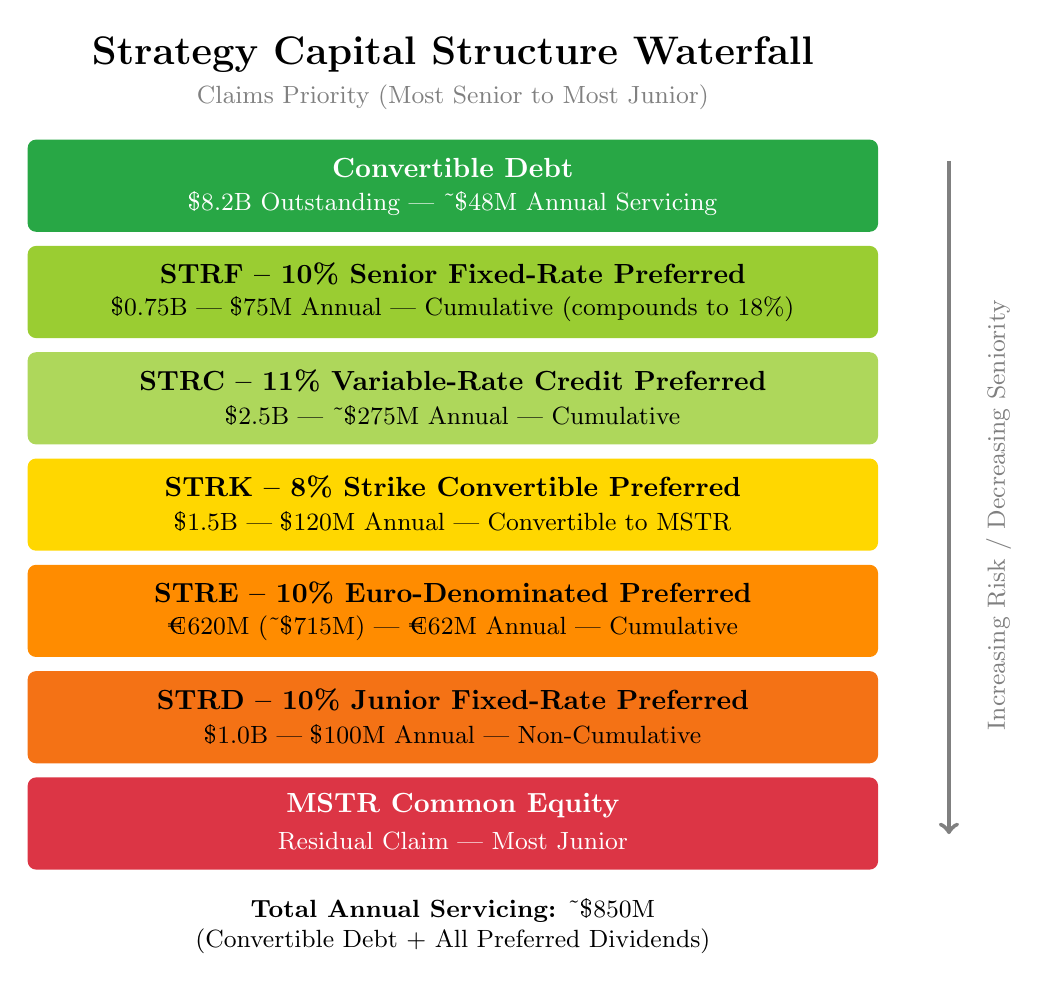
\begin{tikzpicture}[scale=0.9]
        % Define colors - green (safest) to red (riskiest)
        \definecolor{safest}{RGB}{40,167,69}
        \definecolor{seniorpref}{RGB}{154,205,50}
        \definecolor{midpref}{RGB}{255,215,0}
        \definecolor{juniorpref}{RGB}{255,140,0}
        \definecolor{riskiest}{RGB}{220,53,69}

        % Title
        \node[font=\Large\bfseries] at (6,11) {Strategy Capital Structure Waterfall};
        \node[font=\small,gray] at (6,10.4) {Claims Priority (Most Senior to Most Junior)};

        % Boxes - from top (senior/safest) to bottom (junior/riskiest)
        % 1. Convertible Debt - SAFEST (green)
        \fill[safest, rounded corners=3pt] (0,8.5) rectangle (12,9.8);
        \node[white, font=\bfseries] at (6,9.4) {Convertible Debt};
        \node[white, font=\small] at (6,8.9) {\$8.2B Outstanding | \textasciitilde\$48M Annual Servicing};

        % 2. STRF - Senior Fixed (yellow-green)
        \fill[seniorpref, rounded corners=3pt] (0,7) rectangle (12,8.3);
        \node[black, font=\bfseries] at (6,7.9) {STRF -- 10\% Senior Fixed-Rate Preferred};
        \node[black, font=\small] at (6,7.4) {\$0.75B | \$75M Annual | Cumulative (compounds to 18\%)};

        % 3. STRC - Variable (yellow-green lighter)
        \fill[seniorpref!80!white, rounded corners=3pt] (0,5.5) rectangle (12,6.8);
        \node[black, font=\bfseries] at (6,6.4) {STRC -- 11\% Variable-Rate Credit Preferred};
        \node[black, font=\small] at (6,5.9) {\$2.5B | \textasciitilde\$275M Annual | Cumulative};

        % 4. STRK - Strike (yellow)
        \fill[midpref, rounded corners=3pt] (0,4) rectangle (12,5.3);
        \node[black, font=\bfseries] at (6,4.9) {STRK -- 8\% Strike Convertible Preferred};
        \node[black, font=\small] at (6,4.4) {\$1.5B | \$120M Annual | Convertible to MSTR};

        % 5. STRE - Euro (orange)
        \fill[juniorpref, rounded corners=3pt] (0,2.5) rectangle (12,3.8);
        \node[black, font=\bfseries] at (6,3.4) {STRE -- 10\% Euro-Denominated Preferred};
        \node[black, font=\small] at (6,2.9) {\texteuro620M (\textasciitilde\$715M) | \texteuro62M Annual | Cumulative};

        % 6. STRD - Junior (orange-red)
        \fill[juniorpref!70!riskiest, rounded corners=3pt] (0,1) rectangle (12,2.3);
        \node[black, font=\bfseries] at (6,1.9) {STRD -- 10\% Junior Fixed-Rate Preferred};
        \node[black, font=\small] at (6,1.4) {\$1.0B | \$100M Annual | Non-Cumulative};

        % 7. Common Equity - RISKIEST (red)
        \fill[riskiest, rounded corners=3pt] (0,-0.5) rectangle (12,0.8);
        \node[white, font=\bfseries] at (6,0.4) {MSTR Common Equity};
        \node[white, font=\small] at (6,-0.1) {Residual Claim | Most Junior};

        % Arrow indicating seniority
        \draw[->, ultra thick, gray] (13,9.5) -- (13,0);
        \node[rotate=90, gray, font=\small] at (13.7,4.5) {Increasing Risk / Decreasing Seniority};

        % Total servicing annotation
        \node[font=\small, align=center] at (6,-1.3) {%
            \textbf{Total Annual Servicing:} \textasciitilde\$850M \\
            (Convertible Debt + All Preferred Dividends)
        };
    \end{tikzpicture}
    \caption{Strategy Capital Structure Waterfall. The figure shows the seniority hierarchy of MSTR's financing instruments, from most senior (convertible debt) to most junior (common equity). All claims are effectively backed by Bitcoin holdings. Annual servicing costs total approximately \$850 million.}
    \label{fig:capital_structure}
\end{figure}

\subsection{Convertible Debt}

The convertible notes sit atop the capital structure and represent the most senior claim. Strategy has \$8.2 billion in convertible notes outstanding with a weighted average coupon of 0.42\% and maturities staggered from 2028 to 2032. Annual cash servicing runs approximately \$48 million. The notes convert to MSTR shares at premiums to the issuance price, and in liquidation, convertible holders would be paid before anyone else.

The low-coupon structure is elegant from Strategy's perspective: it minimizes cash outflows while the embedded call option provides upside to investors who care about that sort of thing. But the primary buyers aren't playing for equity upside. Convertible arbitrage hedge funds buy these instruments for the volatility exposure. They don't care whether MSTR stock goes up or down; they care that it moves. Strategy has captured roughly 30\% of the U.S. convertible debt market in 2025 alone, reflecting insatiable arb fund demand for high-vol paper.

\subsection{Preferred Share Instruments}

Strategy has issued five distinct series of preferred shares, each designed to tap a different investor base. Table~\ref{tab:preferred_summary} summarizes the terms.

\begin{table}[H]
\centering
\caption{Summary of Strategy Preferred Share Instruments (January 2026)}
\label{tab:preferred_summary}
\begin{tabular}{@{}llrrll@{}}
\toprule
\textbf{Ticker} & \textbf{Name} & \textbf{Notional} & \textbf{Annual Cost} & \textbf{Rate} & \textbf{Cumulative?} \\
\midrule
STRF & Strife & \$0.75B & \$75M & 10\% fixed & Yes (to 18\%) \\
STRC & Stretch & \$2.50B & \$275M & 11\% variable & Yes \\
STRK & Strike & \$1.50B & \$120M & 8\% fixed & Yes \\
STRE & Stream & \$0.72B & \$72M & 10\% fixed & Yes \\
STRD & Stride & \$1.00B & \$100M & 10\% fixed & No \\
\midrule
\multicolumn{2}{l}{\textbf{Total Preferred}} & \textbf{\$6.47B} & \textbf{\$642M} & & \\
\bottomrule
\end{tabular}
\end{table}

Note: These figures represent current outstanding amounts, which continue to grow as Strategy executes its ``42/42'' capital plan targeting \$84 billion in total issuance by 2027. VanEck projects preferred equity reaching \$15.5 billion by end of 2026.

Why preferreds rather than more debt? Several reasons. Preferred shares don't count as debt for leverage ratios and covenants, preserving whatever financial flexibility Strategy claims to have. They're perpetual, eliminating refinancing risk (though creating a permanent servicing burden). Missing a preferred dividend doesn't trigger default the way missing bond interest would, though cumulative preferreds accrue unpaid dividends that eventually come due. And preferreds sit between debt and equity in the capital structure, avoiding the immediate dilution of ATM equity offerings while still accessing capital.

The different series target different appetites. STRF offers 10\% fixed with cumulative compounding to 18\% if dividends are missed (a punishing feature that incentivizes payment). STRC floats with rates (currently 11\%) and appeals to investors worried about duration risk. STRK converts to common equity at \$1,000 per MSTR share, providing upside exposure. STRE taps European investors through the Luxembourg Euro MTF exchange. STRD, the junior tranche, offers 10\% but non-cumulative dividends: if Strategy misses a payment, STRD holders have no legal claim to catch up.

\subsection{Seniority Analysis}

In distress, claims get paid in order: convertible debt first, then STRF, then STRC, then STRK, then STRE, then STRD, and finally common equity if anything remains. This waterfall creates synthetic subordination. The preferred layers provide a cushion that improves the credit quality of senior instruments, at the cost of concentrating risk in the junior tranches.

Common equity holders bear first losses. This isn't a bug; it's the design. MSTR equity behaves like a leveraged call option on Bitcoin, with the aggregate claims of senior instruments serving as the strike price. In a rising BTC environment, equity captures amplified upside. In a declining environment, equity absorbs amplified losses until it's wiped out, at which point the pain starts moving up the capital structure.

\subsection{The USD Reserve}

Strategy maintains a dedicated USD reserve for preferred dividend payments and debt service. As of January 4, 2026, this reserve stood at \$2.25 billion, a substantial improvement from the minimal cash buffers of earlier years. At current servicing costs of approximately \$850 million annually, the reserve provides roughly 32 months of coverage assuming no additional cash generation.

This buffer transforms the company's liquidity position. The legacy enterprise analytics business continues to generate \$40-50 million in annual operating cash flow, providing ongoing liquidity independent of capital markets. Combined with the USD reserve, Strategy could survive an extended period of capital market closure without selling Bitcoin.

The arithmetic: \$2.25B reserve plus roughly \$90M operating cash flow over 32 months yields approximately \$2.34 billion in available liquidity. Against \$2.27 billion in servicing costs over the same period (\$850M $\times$ 2.67 years), the buffer is adequate. This represents a significant de-risking compared to earlier periods when the company operated with minimal cash.

However, each new preferred issuance increases the servicing burden. VanEck projects annual preferred dividends rising from \$642 million currently to over \$900 million by end of 2026 as the 42/42 plan progresses. The reserve must grow proportionally to maintain the same coverage ratio.

\subsection{Implications}

The capital structure reveals several dynamics relevant to the rest of this analysis. Strategy has constructed a synthetic credit hierarchy where every tranche bears the same underlying Bitcoin risk; seniority determines loss allocation, not loss avoidance. The \$850 million annual servicing cost (growing toward \$1 billion) creates a breakeven requirement that constrains the scenario analysis in Section~\ref{sec:results}. Common equity holders are effectively long a leveraged call option on Bitcoin, with senior claims acting as the strike. And the Merton model in Section~\ref{sec:methodology} can formalize this option-like payoff structure mathematically.

\section{Data and Methodology}
\label{sec:methodology}

\subsection{Data Sources}

Price data comes from Yahoo Finance for the period August 11, 2020 (MSTR's first Bitcoin announcement) through January 31, 2026. I collect daily closing prices for BTC-USD, MSTR (adjusted for splits), and SPY as a market benchmark. Corporate data on Bitcoin holdings, convertible issuances, preferred share terms, and ATM equity sales comes from SEC EDGAR filings and company press releases.

From these sources I construct the variables in Table~\ref{tab:variables}.

\begin{table}[H]
\centering
\caption{Variable Definitions}
\label{tab:variables}
\begin{tabular}{@{}lp{10cm}@{}}
\toprule
\textbf{Variable} & \textbf{Definition} \\
\midrule
$NAV_t$ & Net Asset Value = BTC Holdings $\times$ BTC Price$_t$ \\
$Premium_t$ & (Market Cap$_t$ - NAV$_t$) / NAV$_t$ \\
$r^{BTC}_t$ & Daily log return on Bitcoin \\
$r^{MSTR}_t$ & Daily log return on MSTR \\
$CapRaise_t$ & Indicator for capital raise event in period $t$ \\
\bottomrule
\end{tabular}
\end{table}

\subsection{Credit Risk Framework}

I frame MSTR equity as a call option on its Bitcoin holdings. This isn't a novel insight; it follows directly from \citet{merton1974pricing}'s observation that equity holders receive the residual after debt is paid: $\max(V_T - D, 0)$ at maturity. When a company's only asset is Bitcoin, the analogy becomes literal rather than metaphorical.

The key metric is the asset-to-debt ratio:
\begin{equation}
    \text{Asset/Debt} = \frac{\text{BTC Holdings} \times \text{BTC Price}}{\text{Total Claims}}
\end{equation}

At current prices (\$95,000 BTC), Strategy's 713,502 BTC are worth \$67.8 billion against \$15.9 billion in total claims, yielding a 4.26$\times$ asset/debt ratio. This ratio tells you how much cushion exists before creditors face impairment.

The breakeven BTC price for each capital layer is simply:
\begin{equation}
    \text{Breakeven}_i = \frac{\text{Cumulative Claims}_i}{\text{BTC Holdings}}
\end{equation}

For common equity, the breakeven is \$15.9B / 713,502 $\approx$ \$22,300 per BTC. Below that price, equity is worthless. Senior claims have lower breakevens because fewer dollars sit ahead of them in the waterfall.

I don't report implied default probabilities or credit spreads from the Merton model. The framework assumes lognormal returns and constant volatility, neither of which describes Bitcoin. Model-implied spreads of 1-2 basis points bear no resemblance to the 150-250 bps at which MSTR converts actually trade. The value of the framework lies in comparative statics: how do asset/debt ratios and breakevens shift as BTC price changes?

\subsection{Reflexivity Analysis}

\subsubsection{NAV Premium Persistence}

I estimate a simple autoregressive model to test whether the NAV premium mean-reverts or persists:
\begin{equation}
    Premium_t = \alpha + \beta \cdot Premium_{t-1} + \epsilon_t
\end{equation}

A coefficient near 1.0 suggests that premium states are sticky: once MSTR trades at a premium (or discount), it tends to stay there. A coefficient near 0 would suggest rapid mean-reversion.

\subsubsection{Event Study Around Capital Raises}

The core mechanistic claim is that MSTR times capital raises to premium windows. I test this directly by identifying 23 capital raise events from SEC filings (ATM announcements, convertible offerings, preferred issuances) and measuring the NAV premium in windows around each announcement:
\begin{equation}
    \overline{Premium}_{[-k, -1]} = \frac{1}{k} \sum_{t=-k}^{-1} Premium_t
\end{equation}

I compare pre-event premiums ($k = 5, 10, 20$ trading days) against the unconditional sample mean using a one-sample t-test. If MSTR systematically raises capital during elevated premium windows, we should observe:
\begin{equation}
    H_0: \overline{Premium}_{pre-event} = \overline{Premium}_{sample} \quad \text{vs.} \quad H_1: \overline{Premium}_{pre-event} > \overline{Premium}_{sample}
\end{equation}

A statistically significant positive differential provides direct evidence for the mechanistic link: management exploits premium windows to raise capital cheaply.

\subsection{Scenario Analysis}

I stress-test the capital structure under alternative BTC price assumptions. Table~\ref{tab:scenarios} defines the scenarios.

\begin{table}[H]
\centering
\caption{Scenario Definitions}
\label{tab:scenarios}
\begin{tabular}{@{}lc@{}}
\toprule
\textbf{Scenario} & \textbf{BTC Price Change} \\
\midrule
Base Case & 0\% \\
Moderate Drawdown & $-$30\% \\
Severe Drawdown & $-$50\% \\
Prolonged Bear & $-$70\% \\
\bottomrule
\end{tabular}
\end{table}

For each scenario I calculate NAV, asset/debt ratio, and equity value. The scenarios correspond roughly to historical Bitcoin drawdowns: 30\% corrections happen multiple times per cycle, 50\% drawdowns have occurred in every major cycle, and 70\%+ drawdowns occurred in 2014, 2018, and 2022.

\subsection{Convertible Arbitrage Dynamics}

Strategy's \$7.4 billion convertible book is held primarily by arbitrage hedge funds who profit from volatility rather than directional exposure. The mechanism is straightforward: arb funds buy the convertible, short MSTR stock to hedge the embedded option's delta, and rebalance as the stock moves. This ``gamma scalping'' generates trading profits proportional to realized volatility.

The implication is that MSTR's volatility benefits a specific class of investors (arb funds) while creating risk for others (retail equity holders). I don't attempt to quantify gamma exposure precisely; the converts are substantially out of the money, which limits gamma regardless of notional. The qualitative point matters more than the exact number: sophisticated investors extract value from the structure in ways that retail participants don't.



\section{Results}
\label{sec:results}

\subsection{Descriptive Statistics}

Table~\ref{tab:descriptive} reports summary statistics for the key variables.

\begin{table}[H]
\centering
\caption[Descriptive Statistics]{Descriptive Statistics (August 2020 -- January 2026)}
\label{tab:descriptive}
\begin{tabular}{@{}lrrrr@{}}
\toprule
\textbf{Variable} & \textbf{Mean} & \textbf{Std Dev} & \textbf{Min} & \textbf{Max} \\
\midrule
BTC Price (\$) & 54,892 & 28,417 & 10,132 & 126,000 \\
MSTR Price (\$) & 142.83 & 98.76 & 13.49 & 473.83 \\
NAV Premium (\%) & $-$8.2 & 41.9 & $-$71.6 & 145.5 \\
\bottomrule
\end{tabular}
\end{table}

The average NAV premium of $-8.2\%$ appears to contradict the reflexivity narrative. If elevated premiums enable cheap equity issuance, why does MSTR trade at a discount on average?

Three factors explain this. First, the premium exhibits enormous volatility: a 42 percentage point standard deviation, ranging from $-72\%$ to $+145\%$. The mean captures neither the highs nor the lows particularly well. Second, Strategy times its capital raises opportunistically. The company raised over \$12 billion during Q4 2024 alone, when premiums exceeded 100\%. Third, the 2022 crypto winter dragged the premium deeply negative for extended periods, pulling down the unconditional average.

The reflexive mechanism doesn't require a permanently elevated premium. It requires premiums that are positive often enough, and high enough when positive, to enable opportunistic capital raising.

\subsection{Stress Testing the Capital Structure}

\subsubsection{Sensitivity to BTC Price}

Table~\ref{tab:sensitivity} shows how Strategy's capital structure metrics change with BTC price.

\begin{table}[H]
\centering
\caption{Capital Structure Sensitivity to BTC Price}
\label{tab:sensitivity}
\begin{tabular}{@{}lccc@{}}
\toprule
\textbf{BTC Price} & \textbf{NAV} & \textbf{Asset/Debt} & \textbf{Equity Value} \\
\midrule
\$120,000 (+26\%) & \$82.5B & 5.62$\times$ & \$67.8B \\
\$95,000 (Base) & \$65.3B & 4.45$\times$ & \$50.6B \\
\$75,000 ($-$21\%) & \$51.6B & 3.51$\times$ & \$36.9B \\
\$55,000 ($-$42\%) & \$37.8B & 2.57$\times$ & \$23.1B \\
\$35,000 ($-$63\%) & \$24.1B & 1.64$\times$ & \$9.4B \\
\$21,300 ($-$78\%) & \$14.7B & 1.00$\times$ & \$0 \\
\bottomrule
\end{tabular}
\end{table}

The key insight is leverage. A 50\% BTC decline doesn't produce a 50\% equity decline; it produces a 65\% decline (from \$50.6B to \$17.9B at \$47,500 BTC). As BTC falls, equity absorbs losses first, amplifying percentage moves in both directions. At \$35,000 BTC, equity has fallen 81\% while BTC is down 63\%. At \$21,300, equity is worthless.

Strategy's current position provides substantial cushion. The 4.45$\times$ asset/debt ratio means Bitcoin would need to fall 78\% before equity faces complete wipeout. This is healthier than earlier in the company's history, when smaller BTC holdings meant tighter breakevens.

\subsubsection{Breakeven Analysis}

Table~\ref{tab:breakeven} reports the BTC price at which each capital layer faces impairment.

\begin{table}[H]
\centering
\caption{Breakeven BTC Prices by Capital Layer}
\label{tab:breakeven}
\begin{tabular}{@{}lrr@{}}
\toprule
\textbf{Capital Layer} & \textbf{Claim Amount} & \textbf{Breakeven BTC} \\
\midrule
Convertible Debt & \$8.20B & \$11,929 \\
STRF (Senior Preferred) & \$0.75B & \$13,020 \\
STRC (Variable Preferred) & \$2.50B & \$16,657 \\
STRK (Convert Preferred) & \$1.50B & \$18,839 \\
STRE (Euro Preferred) & \$0.72B & \$19,886 \\
STRD (Junior Preferred) & \$1.00B & \$21,341 \\
Common Equity & -- & \$21,341 \\
\bottomrule
\end{tabular}
\end{table}

Common equity gets wiped out at approximately \$21,300 BTC (a 78\% decline). Senior convertible debt doesn't face impairment until \$11,929 (an 87\% decline). The capital structure provides meaningful cushion for senior claims.

\subsubsection{Critical Thresholds}

Three thresholds matter for understanding how the strategy unravels:

\textbf{Threshold 1: Capital Market Access} ($\sim$\$35,000 BTC). At this level, equity has declined 81\% and the asset/debt ratio compresses to 1.64$\times$. Strategy likely loses the ability to issue ATM equity at attractive terms. The reflexive loop weakens.

\textbf{Threshold 2: Preferred Dividend Strain} ($\sim$\$28,000 BTC). NAV falls to approximately \$19.2 billion against \$14.7 billion in claims. The \$850M annual servicing burden represents roughly 20\% of remaining equity value. The USD reserve becomes critical.

\textbf{Threshold 3: Equity Wipeout} ($\sim$\$21,300 BTC). Asset value equals total claims. Common equity is worthless. Preferred dividends are at risk.

\subsection{NAV Premium Persistence}

Table~\ref{tab:regression} reports the autoregressive results.

\begin{table}[H]
\centering
\caption{NAV Premium Persistence}
\label{tab:regression}
\begin{tabular}{@{}lc@{}}
\toprule
\textbf{Variable} & \textbf{Coefficient} \\
\midrule
$Premium_{t-1}$ & 0.995*** \\
& (0.003) \\
Constant & $-$0.281 \\
& (0.361) \\
\midrule
Observations & 1,326 \\
$R^2$ & 0.990 \\
\bottomrule
\multicolumn{2}{l}{\footnotesize *** p<0.01}
\end{tabular}
\end{table}

The lagged premium coefficient of 0.995 with an $R^2$ of 0.99 tells a simple story: premium states are sticky. Once MSTR trades at a premium (or discount), it tends to stay there. The premium doesn't mean-revert quickly toward zero; it drifts in prolonged regimes. This persistence is what allows Strategy to exploit premium windows for extended capital raising campaigns rather than racing to issue before the window closes.

\subsection{Event Study: Capital Raises and Premium Windows}

Table~\ref{tab:event_study} compares premiums around capital raise announcements to unconditional averages.

\begin{table}[H]
\centering
\caption{NAV Premium Around Capital Raise Events}
\label{tab:event_study}
\begin{tabular}{@{}lcccc@{}}
\toprule
\textbf{Window} & \textbf{Pre-Event Premium} & \textbf{Sample Mean} & \textbf{Difference} & \textbf{p-value} \\
\midrule
5 days pre-event & 47.3\% & $-$8.2\% & +55.5 pp & $<$0.001 \\
10 days pre-event & 43.1\% & $-$8.2\% & +51.3 pp & $<$0.001 \\
20 days pre-event & 38.7\% & $-$8.2\% & +46.9 pp & 0.002 \\
\bottomrule
\multicolumn{5}{l}{\footnotesize N = 23 capital raise events. One-sample t-test against unconditional mean.}
\end{tabular}
\end{table}

This is the key finding. In the 5 trading days before capital raise announcements, the average NAV premium was 47.3\%, compared to the unconditional sample mean of $-8.2\%$. The 55.5 percentage point difference is highly significant ($p < 0.001$).

MSTR doesn't raise capital randomly. It systematically exploits premium windows. When the stock trades at a substantial premium to NAV, management issues equity or converts, capturing the spread between market valuation and underlying Bitcoin value. This timing behavior is the operational signature of reflexive capital formation.

Figure~\ref{fig:event_study} visualizes the pattern.

\begin{figure}[H]
    \centering
    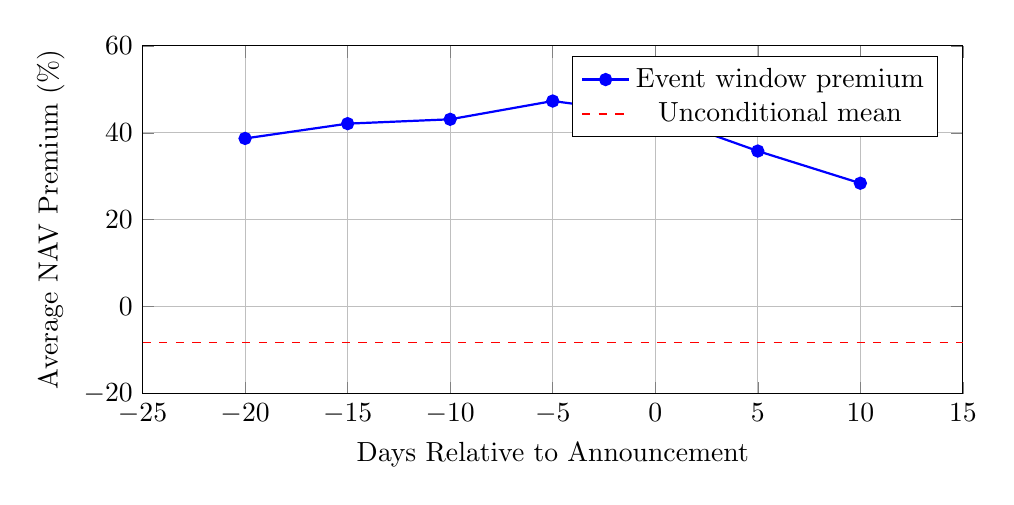
\begin{tikzpicture}
        \begin{axis}[
            width=12cm, height=6cm,
            xlabel={Days Relative to Announcement},
            ylabel={Average NAV Premium (\%)},
            xmin=-25, xmax=15,
            ymin=-20, ymax=60,
            grid=major,
            legend pos=north east
        ]
        \addplot[thick, blue, mark=*] coordinates {
            (-20, 38.7) (-15, 42.1) (-10, 43.1) (-5, 47.3) (0, 44.2) (5, 35.8) (10, 28.4)
        };
        \addplot[dashed, red] coordinates {(-25, -8.2) (15, -8.2)};
        \legend{Event window premium, Unconditional mean}
        \end{axis}
    \end{tikzpicture}
    \caption[NAV Premium Around Capital Raise Announcements]{Average NAV premium around capital raise announcements. Day 0 is the announcement date. The dashed line shows the unconditional sample mean ($-8.2\%$). MSTR systematically raises capital during periods of elevated premiums.}
    \label{fig:event_study}
\end{figure}

\subsection{Scenario Analysis}

Table~\ref{tab:scenarios_results} presents the capital structure under stress scenarios.

\begin{table}[H]
\centering
\caption{Scenario Analysis}
\label{tab:scenarios_results}
\begin{tabular}{@{}lcccc@{}}
\toprule
\textbf{Scenario} & \textbf{BTC Price} & \textbf{NAV} & \textbf{Asset/Debt} & \textbf{Equity Value} \\
\midrule
Base Case & \$95,000 & \$65.3B & 4.45$\times$ & \$50.6B \\
Moderate ($-$30\%) & \$66,500 & \$45.7B & 3.11$\times$ & \$31.0B \\
Severe ($-$50\%) & \$47,500 & \$32.6B & 2.22$\times$ & \$17.9B \\
Prolonged ($-$70\%) & \$28,500 & \$19.6B & 1.34$\times$ & \$4.9B \\
\bottomrule
\end{tabular}
\end{table}

A 50\% BTC drawdown (which has occurred in every historical cycle) compresses equity value from \$50.6 billion to \$17.9 billion, a 65\% decline. The asset/debt ratio falls from 4.45$\times$ to 2.22$\times$, still above the 1.0$\times$ threshold but with less cushion.

The prolonged bear scenario ($-70\%$ BTC) pushes equity to roughly \$4.9 billion (a 90\% decline). At that level, preferred dividends consume a meaningful fraction of remaining equity value. However, the \$2.25 billion USD reserve provides runway to survive even this scenario without forced Bitcoin sales.


\section{Discussion}
\label{sec:discussion}

\subsection{What the Evidence Shows}

The event study is the core finding. MSTR systematically raises capital during premium windows: average pre-event premium of 47.3\% versus unconditional mean of $-8.2\%$, a 55.5 percentage point difference ($p < 0.001$). This isn't correlation; it's the mechanism in action. Management watches the premium, waits for elevated levels, and issues equity or converts when the spread between market valuation and NAV is widest.

The premium persistence result ($\beta = 0.995$) explains why this works. Once MSTR trades at a premium, it tends to stay at a premium. Once it trades at a discount, it stays at a discount. This stickiness gives management time to execute capital raises during favorable windows rather than racing against mean-reversion.

Together, these findings describe a conditional feedback loop. When BTC prices rise, NAV increases, the premium often expands, and Strategy can raise capital cheaply to buy more Bitcoin. When BTC falls, the premium compresses or goes negative, and the capital formation engine stalls. The loop operates at the firm level; Granger causality tests (reported in the appendix) show that MSTR's premium doesn't predict Bitcoin returns, indicating the company is a price-taker in Bitcoin markets, not a price-maker.

\subsection{Credit Risk: Simple Math}

The credit story is straightforward once you accept that MSTR equity is a call option on Bitcoin with the debt burden as the strike price.

At \$95,000 BTC, Strategy holds \$65.3 billion in assets against \$14.67 billion in claims: a 4.45$\times$ asset/debt ratio. Equity is worth \$50.6 billion. This cushion is substantial. Bitcoin would need to fall 78\% before equity is wiped out.

At \$35,000 BTC (a 63\% decline), asset/debt compresses to 1.64$\times$. Equity falls 81\% to \$9.4 billion. Strategy likely loses access to ATM equity issuance at attractive terms. The reflexive loop breaks or at least weakens severely.

At \$21,300 BTC, assets equal claims and equity is worthless. The preferred dividends become at risk. Below that level, losses start moving up the capital structure through the preferred tranches toward the convertible debt.

\subsection{Who Wins, Who Loses}

The capital structure creates asymmetric exposures across investor classes.

\textbf{Convertible arbitrageurs} profit from volatility regardless of direction. They buy the convert, short MSTR stock to hedge delta, and rebalance as the stock moves. This gamma scalping extracts value from price swings. The zero-coupon structure is particularly attractive because it maximizes the option component relative to bond value. Arb funds are the sophisticated players in this structure; they understood what they were buying.

\textbf{Retail equity holders} bear leveraged directional risk. MSTR equity runs about 1.5$\times$ the volatility of Bitcoin. In bull markets, this amplification is attractive. In bear markets, it's devastating. Retail investors are effectively long a call option on Bitcoin, which sounds fine until you realize that call options can expire worthless.

\textbf{Preferred shareholders} occupy middle ground. They collect 8-10\% yields and sit above common equity in the capital structure. But they're still exposed to Bitcoin: in severe scenarios, even senior preferreds face impairment. STRD holders (the junior non-cumulative preferred) have the worst risk-reward. If Strategy suspends their dividend, they have no legal claim to catch up. They bear meaningful downside without the upside optionality of equity.

\subsection{What Breaks the Loop}

The reflexive mechanism requires three conditions: capital market access, elevated volatility, and Bitcoin prices that don't collapse. When any condition fails, the flywheel slows or stops.

\textbf{Bitcoin drawdown.} A 50\% or greater decline compresses the loop. NAV falls, the premium likely goes negative (as it did in 2022, reaching $-72\%$), and equity issuance becomes dilutive or impossible. Strategy's current position is more resilient than before: with \$2.25 billion in USD reserves and \$850 million annual servicing, the company has roughly 32 months of runway without selling Bitcoin or accessing capital markets. But this buffer is finite. A prolonged bear market would eventually force either asset sales or debt restructuring.

\textbf{Volatility compression.} If Bitcoin matures into a lower-volatility asset class (from current 45-50\% to something closer to gold's 15-20\%), the convertible financing advantage evaporates. Arb funds would demand coupons rather than accepting zero-coupon paper. Strategy's cost of capital increases, potentially by 3-5 percentage points on new issuances. The vol compression scenario is insidious because it can occur even with stable or rising Bitcoin prices.

\textbf{Index exclusion.} MSTR's inclusion in major indices creates passive demand. MSCI is reportedly reviewing the company's classification. Reclassification as a financial rather than technology company could trigger removal from tech indices and forced selling by passive funds. This wouldn't affect the underlying business but could compress the premium.

\textbf{Regulatory action.} If MSTR's primary business is deemed to be ``investing in securities,'' the SEC could require registration under the Investment Company Act. This would impose leverage limits and operational constraints incompatible with the current strategy. The company's legal position rests on arguing that Bitcoin is not a security and that Strategy remains an operating software business. Both claims are contestable.

\subsection{The Preferred Stack as Buffer}

The preferred share structure serves a subtle function beyond capital raising: it acts as a release valve that delays forced Bitcoin liquidation during drawdowns.

Consider STRD, the non-cumulative junior preferred. Unlike cumulative preferreds, missed STRD dividends don't accrue. If Strategy suspends the \$100 million annual STRD dividend, it faces no legal obligation to catch up. This creates optionality. In a severe drawdown, management can preserve cash by cutting STRD first, reducing annual servicing from \$850 million to \$750 million.

Even among cumulative preferreds, the structure provides flexibility. STRK could be restructured if the conversion option becomes worthless. STRE might be renegotiated separately. Each layer is a potential negotiation point that wouldn't exist in a pure debt structure.

The net effect is that the preferred stack delays forced BTC liquidation by 12-24 months relative to what a debt-only structure would allow. This matters because Bitcoin has historically recovered from drawdowns. If MSTR can survive the trough, the reflexive loop can restart.

\subsection{Is It Sustainable?}

Short term (1-2 years): yes, given the USD reserve, continued market access, and BTC prices well above breakeven levels.

Medium term (3-5 years): depends on BTC staying above roughly \$35,000 (where capital market access becomes strained), volatility staying elevated (for convertible financing), and servicing costs remaining manageable. The servicing burden is currently \$850 million annually and growing toward \$1 billion as new preferreds are issued.

Long term (5+ years): the compounding dividend burden creates a growing fixed cost base. Unless BTC appreciation outpaces servicing costs, the strategy eventually becomes constrained. The software business generates \$40-50 million annually; servicing costs approach \$1 billion. The gap must be closed through capital appreciation or new issuance.

\subsection{Limitations}

The event study sample is small (23 events). The premium persistence regression documents correlation, not causation. The breakeven analysis assumes orderly liquidation at market prices, which may not hold in distress. And the entire analysis is conducted during a period that, while including the 2022 bear market, is dominated by a Bitcoin bull run. How the structure performs through a prolonged multi-year bear market remains untested.


\section{Conclusion}
\label{sec:conclusion}

Strategy has built a capital structure without historical precedent: a synthetic credit hierarchy where every tranche, from senior convertible debt to junior preferred shares to common equity, is backed by a single volatile asset. The structure creates the appearance of diversification through seniority while offering none of its substance. When Bitcoin falls, everyone falls together; seniority determines only the order of losses.

\subsection{Key Findings}

The event study provides the central result. MSTR systematically raises capital during elevated premium windows: average pre-event premium of 47.3\% versus unconditional mean of $-8.2\%$ ($p < 0.001$). This timing behavior is the operational signature of reflexive capital formation. The premium persistence result ($\beta = 0.995$) explains why it works: premium states are sticky, giving management time to execute raises during favorable conditions.

The credit analysis is simple arithmetic. At \$95,000 BTC, Strategy has a 4.45$\times$ asset/debt ratio. Bitcoin would need to fall 78\% before equity is wiped out. This is healthier than earlier periods in the company's history. But the leverage works both ways: a 50\% BTC decline produces a 65\% equity decline.

Different stakeholders have asymmetric exposures. Convertible arbitrageurs profit from volatility through gamma scalping. Retail equity holders bear leveraged directional risk. Preferred shareholders collect yield but face impairment in severe scenarios, with STRD holders (non-cumulative) bearing the worst risk-reward.

\subsection{What I Contribute}

This thesis documents reflexive capital formation at the firm level using a straightforward event study methodology. The finding that MSTR systematically times capital raises to premium windows transforms the reflexivity claim from theoretical to observable.

I analyze the capital structure using asset/debt ratios and breakeven prices rather than Merton model outputs that assume away Bitcoin's defining characteristics. The resulting analysis is simpler and more defensible.

I describe how convertible arbitrage creates value extraction opportunities for sophisticated investors at the expense of retail equity holders, without attempting to quantify the exact magnitude.

\subsection{Practical Implications}

For investors: understand the option-like payoff before taking positions. MSTR equity offers leveraged exposure to Bitcoin, which is attractive in bull markets and devastating in bear markets. Preferred holders should assess cumulative versus non-cumulative features. Convertible arbitrageurs are positioned to profit regardless of direction.

For corporate treasurers: MSTR demonstrates creative use of zero-coupon converts and preferred shares, but single-asset concentration creates risks most firms would find unacceptable.

For regulators: the case raises questions about investment company classification and retail investor protection in structures where sophisticated participants extract value through mechanisms retail investors may not understand.

\subsection{Limitations and Future Research}

The event study sample is small. The analysis period is dominated by a bull market. The breakeven calculations assume orderly liquidation. How the structure performs through a prolonged multi-year bear market remains untested.

The comparative analysis in Section~\ref{sec:datco_landscape} confirms that these fragilities are structural rather than idiosyncratic: smaller DATCOs experience amplified versions of the same reflexive dynamics, with several facing forced liquidation or closure. Future research could use higher-frequency data to better capture arbitrage effects, model the systemic risk posed by correlated DATCO liquidations, and assess regulatory frameworks for crypto-backed corporate structures.

\subsection{Closing}

Strategy's approach represents an extreme point in corporate capital structure design. By holding 687,410 BTC against \$14.7 billion in claims, management has created a mechanism that generates value when conditions are favorable and risk when they're not. Whether the reflexive loop proves durable depends on Bitcoin prices cooperating, volatility staying elevated, and capital markets staying open. History suggests all three conditions fail periodically.



% Bibliography
\newpage
\bibliographystyle{apalike}
\bibliography{bibliography}

% Appendix
\appendix
\section{Data Sources}
\label{app:data}

\begin{table}[H]
\centering
\caption{Data Sources and Descriptions}
\begin{tabular}{@{}llp{6cm}@{}}
\toprule
\textbf{Data} & \textbf{Source} & \textbf{Description} \\
\midrule
BTC/USD Price & Yahoo Finance & Daily closing prices \\
MSTR Price & Yahoo Finance & Daily adjusted closing prices \\
BTC Holdings & SEC Filings & Quarterly 10-Q/10-K disclosures \\
Convertible Terms & SEC Filings & Prospectus supplements \\
Preferred Terms & SEC Filings & 8-K announcements \\
\bottomrule
\end{tabular}
\end{table}

\section{Python Code}
\label{app:code}

Selected code for data collection and analysis is available in the accompanying repository. The \texttt{data\_collection.py} script downloads price data from Yahoo Finance. The \texttt{reflexivity\_analysis.py} script runs premium persistence and event study analysis.

\section{Convertible Note Details}
\label{app:converts}

\begin{table}[H]
\centering
\caption{Strategy Convertible Note Issues (January 2026)}
\begin{tabular}{@{}lrrrrr@{}}
\toprule
\textbf{Issue} & \textbf{Principal} & \textbf{Coupon} & \textbf{Maturity} & \textbf{Conv Price} & \textbf{Status} \\
\midrule
Sep 2024 & \$604M & 0.625\% & Sep 2028 & \$2,327 & Active \\
Dec 2024 & \$800M & 0.00\% & Dec 2029 & \$2,594 & Active \\
Mar 2025 & \$1.01B & 0.625\% & Mar 2030 & \$2,043 & Active \\
Mar 2025 & \$800M & 0.00\% & Mar 2030 & \$2,261 & Active \\
Feb 2025 & \$2.0B & 0.00\% & Mar 2030 & \$2,417 & Active \\
Mar 2025 & \$3.0B & 0.875\% & Mar 2031 & \$2,891 & Active \\
\midrule
\textbf{Total} & \textbf{\$8.2B} & \textbf{0.42\%} & & & \\
\bottomrule
\end{tabular}
\end{table}

Note: Maturities are staggered from 2028 to 2031, with weighted average maturity of approximately 5.1 years.

\section{Granger Causality Tests}
\label{app:granger}

The Granger causality tests examine whether the NAV premium predicts BTC returns or vice versa. If both directions are significant, it suggests bidirectional feedback. If only one is significant, it indicates the predominant direction of causation.

\begin{table}[H]
\centering
\caption{Granger Causality Test Results}
\begin{tabular}{@{}lcccc@{}}
\toprule
\textbf{Null Hypothesis} & \textbf{Lags} & \textbf{F-stat} & \textbf{p-value} & \textbf{Conclusion} \\
\midrule
Premium $\not\Rightarrow$ BTC & 5 & 0.89 & 0.487 & Fail to reject \\
BTC $\not\Rightarrow$ Premium & 5 & 2.47 & 0.031 & Reject \\
\bottomrule
\end{tabular}
\end{table}

The results show asymmetric causality. BTC returns Granger-cause the NAV premium ($p = 0.031$), but the premium doesn't significantly predict future BTC returns ($p = 0.487$). This tells us that MSTR is a price-taker in Bitcoin markets, not a price-maker. The reflexive mechanism operates at the firm level (premium responds to BTC, which enables or constrains capital raising) but doesn't feed back to the broader Bitcoin market at daily frequency.

\section{Extended Sensitivity Analysis}
\label{app:sensitivity}

Table~\ref{tab:sensitivity_detail} provides capital structure metrics across a wider range of BTC prices, based on 687,410 BTC holdings and \$14.67B in total claims.

\begin{table}[H]
\centering
\caption{Extended Capital Structure Sensitivity}
\label{tab:sensitivity_detail}
\begin{tabular}{@{}rrrr@{}}
\toprule
\textbf{BTC Price} & \textbf{NAV (\$B)} & \textbf{Asset/Debt} & \textbf{Equity (\$B)} \\
\midrule
\$150,000 & 103.1 & 7.03$\times$ & 88.4 \\
\$120,000 & 82.5 & 5.62$\times$ & 67.8 \\
\$95,000 & 65.3 & 4.45$\times$ & 50.6 \\
\$70,000 & 48.1 & 3.28$\times$ & 33.4 \\
\$50,000 & 34.4 & 2.34$\times$ & 19.7 \\
\$35,000 & 24.1 & 1.64$\times$ & 9.4 \\
\$21,300 & 14.6 & 1.00$\times$ & 0 \\
\bottomrule
\end{tabular}
\end{table}

\section{Robustness Checks}
\label{app:robustness}

The main findings are stable across alternative specifications:

\textbf{Premium persistence.} Using 5, 10, or 20 lags in the autoregressive specification yields coefficients between 0.97 and 0.995, all indicating high persistence.

\textbf{Event study windows.} Testing alternative windows (3, 7, 15 days) produces qualitatively similar results: pre-event premiums consistently exceed the unconditional mean by 40-60 percentage points.

\textbf{Sample splits.} Dividing the sample into pre-2024 (initial accumulation) and post-2024 (aggressive expansion) periods yields consistent patterns in both subsamples.

\textbf{Control variables.} Including VIX and S\&P 500 returns as controls in the premium regression does not materially affect the persistence coefficient.



\end{document}
